\section{Evaluation}

Our testbed consists of four machines, where a single
server plays the role of both Clover memory server (MS) and metadata
server (DN).  Two machines are configured as Clover clients, and the
last hosts our DPDK-based TOR.  Physically, the machines
are identical: each is equipped with two Intel Xeon E5-2640 CPUs and
256~GB of main memory evenly spread across the NUMA domains. Each
server communicates using a Mellanox ConnectX-5 100-Gbps NIC installed
in a 16x PCIe slot interconnected via a 100-Gbps Mellanox Onyx Switch.
All Clover servers are configured with default routing settings:
clients send directly to the metadata and data server.  We install
OpenFlow rules on the Onyx switch to redirect the Clover RDMA traffic
to the DPDK server.

\subsection{Conflict resolution}

We test the performance gains of resolving write conflicts using our
caching TOR. Clover clients are configured to run a YCSB-A benchmark,
50\% read, 50\% write for 1 million requests. Requests for keys are
based on a Zipf distribution generated with an \textit{s} value of
0.75.\todo{show exactly what this means}. In each experiment the
number of client threads is increased which in turn increases the load
on the system. Clover requests are blocking; thus, the throughput is a
factor of both the request latency and the number of client
threads. Figure~\ref{fig:throughput} compares the performance of
native Clover (plotted in red) against our in-network conflict
resolution (hatched blue).

As the number of clients increases so too does the probability that
two client threads will make concurrent writes to the same key. The
number of conflicts resolved in flight directly correlates to
throughput improvements as each successful request reduces the
multiple round trips necessary to resolve write conflicts. Our current
implementation provides a $1.42\times$ throughput improvement at 64
client threads.

Throughput is limited by the scale of our experimental setup, i.e more
client machines can produce higher throughputs.  \todo{This is the
  speculation part we should cut}.  The number of in-flight conflicts
is also effected by the Zipf distribution. We use a Zipf of 0.75,
however a Zipf of 1.0 would result in a distribution skewed towards
fewer keys, which in turn results in more conflicts. Moreover, we find
that Clover's current design leads to hardware contention on the
servers themselves.  In particular, ConnectX-5 NIC performance
degrades as the number of RDMA compare-and-swap operations to the same
memory region across different queue pairs
increases~\cite{design-guidelines}. As our design eliminates the need
for compare-and-swap operations on cached keys, future work will seek
to reduce or eliminate c\&s operations by replacing them at the TOR
with low overhead RDMA writes.

\begin{figure}
    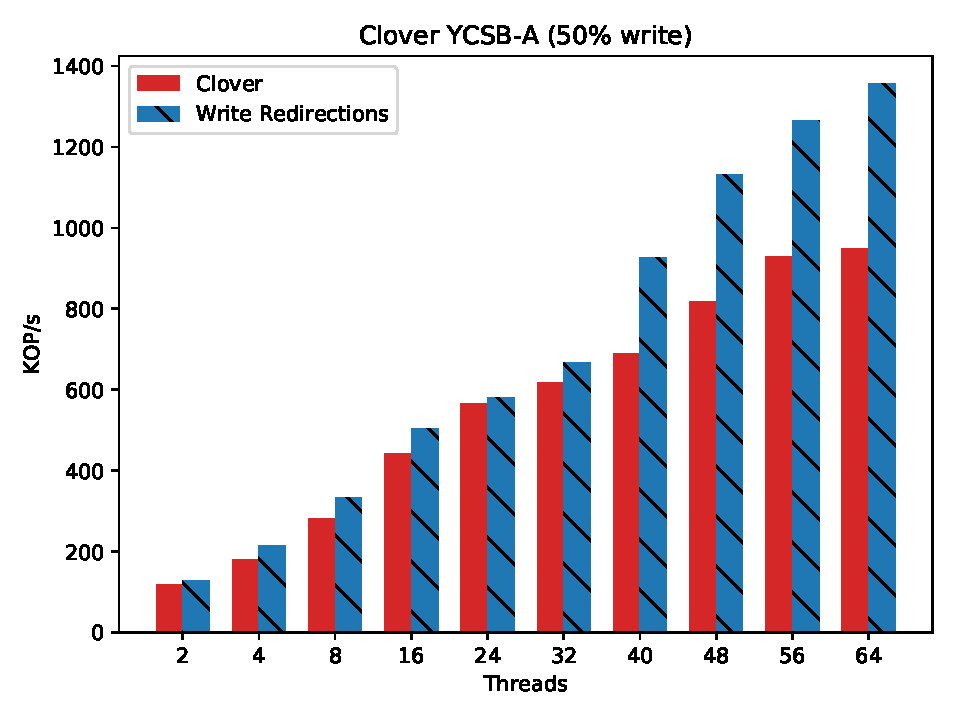
\includegraphics[width=0.45\textwidth]{fig/throughput.pdf}
    \caption{Default Clover throughput vs Clover with write conflict
    detection and correction turned on.}
    \label{fig:throughput}
\end{figure}

\subsection{Memory consumption}

Resources on networking hardware is scarce. High end SoC SmartNIC's
have just a few gigabytes of RAM, and programmable switches have only
megabtyes of SRAM. Moreover the use of this memory is not free: using
memory for any purpose other than buffering packets has a direct
performance cost.
%as the number of packets which can be successfully
%buffered drops. Our design takes the preciousness of memory in network
%into account.
The metadata we cache in network is minimal:
%necessary to resolve write conflicts. While Clover's meta data
%consists of many MB of garbage collection and version data
we only
cache the virtual address of the last write per key,
%In addition we track
as well as the last key written per client. Clients are not
explicitly known to our middlebox and are identified at runtime by
their QP. Tracking clients in this way is necessary to detect write
conflicts in clover. This overhead could be eliminated by explicitly
adding key information to c\&s requests.
%
Figure~\ref{fig:memory} Shows the memory overhead as a function of
keys. Note that 100~K keys can be supported using 7\% of the available
memory on a Barefoot Tofino programmable switch (22~MB).

\begin{figure}
    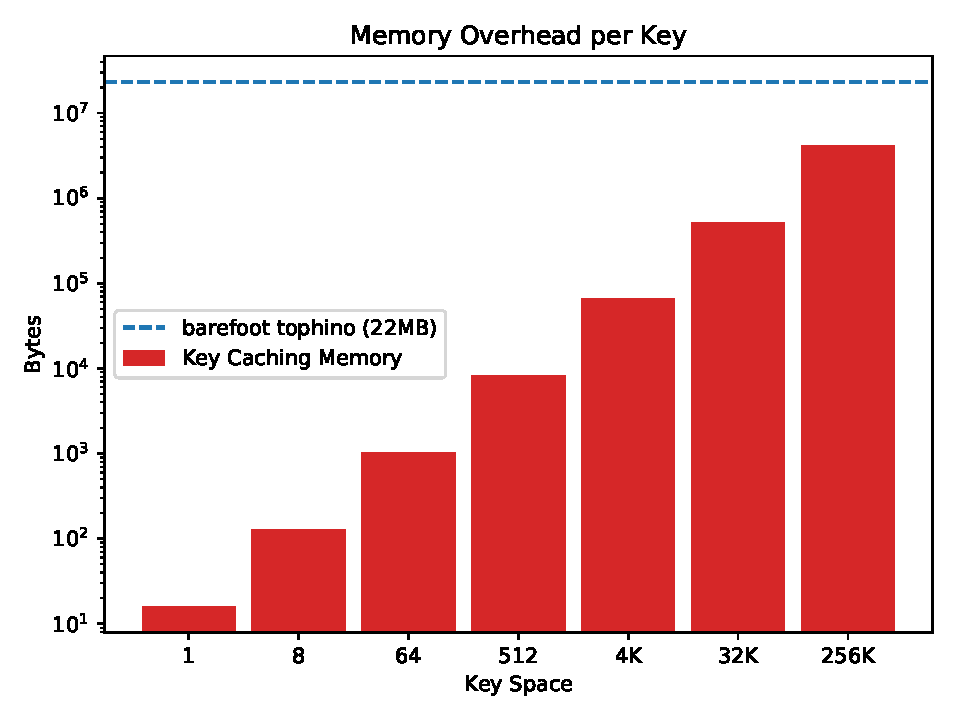
\includegraphics[width=0.45\textwidth]{fig/memory.pdf}
    \caption{Cost of caching metadata in network vs keyspace size.}
    \label{fig:memory}
\end{figure}
\begin{figure}
    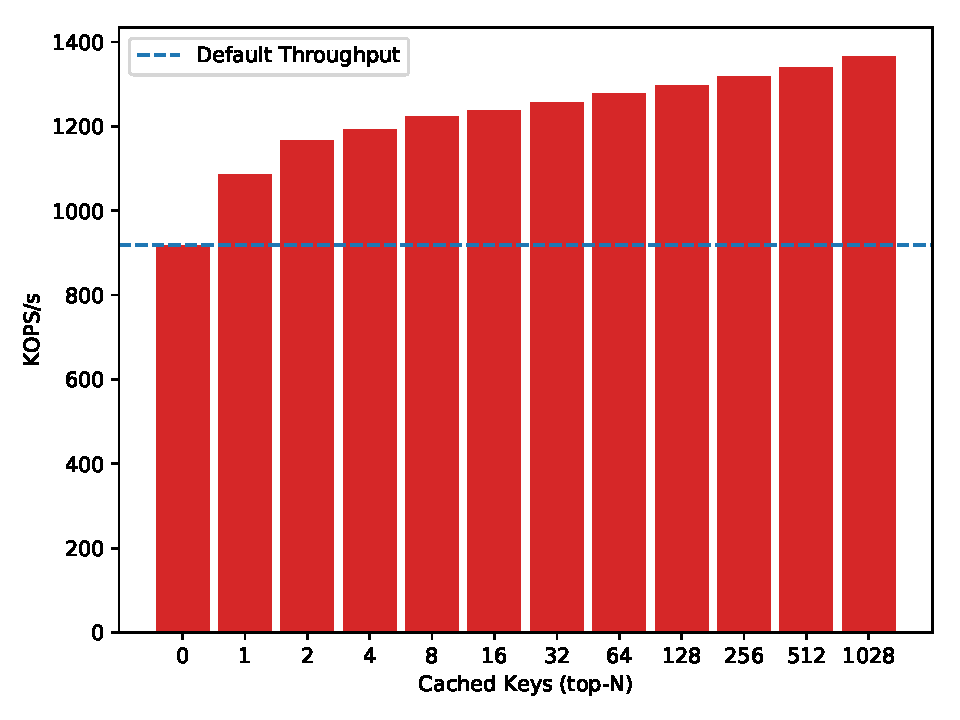
\includegraphics[width=0.45\textwidth]{fig/cache.pdf}
    \caption{Performance as a function of keys cached. Caching a few
    of the top n keys provides the greatest marginal throughput
    benefits.}
    \label{fig:cache}
\end{figure}

%\subsection{Caching top \textit{N} keys} 
%%
Hot keys are the most likely to
contribute to conflict.
%Caching only hot keys results in relatively
%large performance gains while requiring only a small portion of the
%memory required to cache the entire keyspace.
We test the effect of
caching only hot keys by restricting our in-network cache to track and
resolve conflicts on only the top-\textit{N} keys. In this experiment
RDMA requests for keys which are not cached pass through our DPDK TOR
without modification; conflicts are resolved using Clover's existing
reconciliation protocol. Figure~\ref{fig:cache} shows
the throughput for 64 client threads when caching the top-N keys out of a total keyspace size of 1024 keys. The request
distribution is Zipf(0.75), therefore the vast majority of conflicts
occur on the top-eight keys. The in-network memory requirement for eight keys
is 128 bytes, which results in $1.3\times$ throughput improvement.


